\documentclass[11pt]{sdm_internship}
\usepackage[british]{babel}

\usepackage{graphicx}
\graphicspath{{../img/}}

\usepackage{caption}
\usepackage{subcaption}
\usepackage{cleveref}
\usepackage{comment}
\usepackage{wrapfig}
\usepackage{amsfonts}
\usepackage{textcomp}
\usepackage{cprotect}

\pagestyle{plain}

\usepackage{hyperref}
\usepackage{url} \urlstyle{sf}
\newcommand{\email}[1]{\href{mailto:#1}{#1}}

\usepackage{xspace}

\usepackage[dvipsnames]{xcolor}
\newcommand{\addref}[1]{\colorbox{TealBlue!100}{\textcolor{white}{\textbf{$[$\ifx&#1&\ \else#1\fi$]$}}}}
\newcommand{\todo}[1]{\colorbox{Red!75}{\textcolor{white}{\textbf{TODO\ifx&#1&\else: #1\fi}}}}
\newcommand{\rephrase}[1]{\colorbox{BlueViolet!60}{\textcolor{white}{\textbf{$\sim$#1}}}}
\newcommand{\done}{\colorbox{YellowGreen!100}{\textcolor{white}{\textbf{DONE}}}}
\newcommand{\review}{\colorbox{YellowOrange!100}{\textcolor{white}{\textbf{REVIEW}}}}

\newcommand{\dspot}{DSpot\xspace}

\usepackage[newfloat]{minted}
% \usepackage{inconsolata}
% \setmonofont{Inconsolatazi4}

\usepackage{ragged2e}

\usepackage{amsthm}
\theoremstyle{definition}
\newtheorem{definition}{Definition}[section]

\title{Adapting Amplified Unit Tests for Human Comprehension}

\author{Simon \textsc{Bihel}}
\supervisorOne{Benoit \textsc{Baudry}}
\supervisorTwo{~}
\team{KTH Royal Institute of Technology}
\school{ens-Rennes}

\domain{Domain: Software Engineering --- Artificial Intelligence}

\abstract{%
  \justify{%
    \todo{}
  }
}


% Ought to be between 30 and 50 pages

\begin{document}
\maketitle

% ================================================================================
\section*{Introduction}%
\label{sec:intro}%
\addcontentsline{toc}{section}{\nameref{sec:intro}}
\todo{}


% ================================================================================
\section{Background}%
\label{sec:background}
In this section, we present the landscape this thesis fits into.
We define testing (Section~\ref{ssec:software_testing}) as well as go over its use in the industry.
In particular, to understand the needs of practitioners, we present how they assess the quality of their code (Sections~\ref{ssec:elementary_metrics} and~\ref{ssec:mutation_testing}) and what it takes for a new tool to be incorporated in their workflow (Sections~\ref{ssec:need_easy} and~\ref{ssec:cognitive_support_unit_test}).

% --------------------------------------------------------------------------------
\subsection{Software Testing}%
\label{ssec:software_testing}
In this section we give a definition for the test activities and their actors, the different abstraction levels of tests, and our precise object of study, unit tests.

\todo{say the Section~\ref{sssec:test_activities} is a list of definitions to which the reader can refer to later on?}

\todo{Why are we testing software and how do we do it}

\todo{Say that the formal definitions aren't totally necessary}

% - - - - - - - - - - - - - - - - - - - - - - - - - - - - - - - - - - - - - - - -
\subsubsection{Test Activities}%
\label{sssec:test_activities}
\todo{the text is too close to the oracle survey}

Testing is about verifying that a system, for a given scenario, follows a certain behaviour that was previously defined.
The \emph{System-Under-Test} (SUT), in our domain a software system, has a set of components $C$.
A scenario is sequence of stimuli that target a subset of $C$, and trigger responses: (i) feedbacks from the SUT\@; and (ii) changes in the state of its components.
From~\cite{barr2015oracle}, we use the following definition for to combination of stimuli and responses:

\begin{definition}[Test Activities]
  For the SUT $p$, $S$ is the set of stimuli that trigger or constrain $p$'s computation and $R$ is the set of observable responses to a stimulus of $p$.
  $S$ and $R$ are disjoint.
  Test activities form the set $A = S\uplus{}R$.
  The disjoint union is used to label the elements of $A$.
\end{definition}

\begin{wrapfigure}[15]{R}{22em}
  \centering
  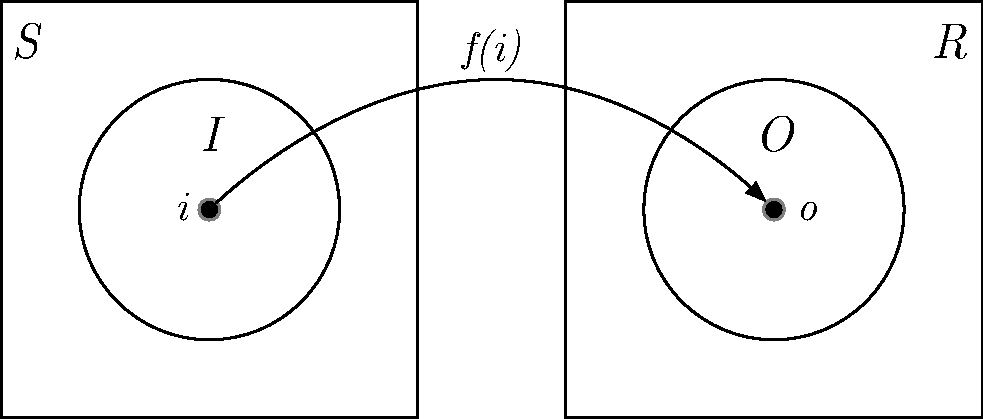
\includegraphics[width=22em]{stim_and_obs}
  \caption{Stimuli and observations: $S$ is anything that can change the observable behaviour of the SUT $f$; $R$ is anything that can be observed about the system's behaviour; $I$ includes $f$'s explicit inputs; $O$ is its explicit outputs; everything not in $S \cup R$ neither affects nor is affected by $f$.}%
  \label{fig:test_activity}
\end{wrapfigure}

The use of the terms ``stimulus'' and ``observations'' fits various test scenarios, functional and non-functional.
As depicted in \figurename~\ref{fig:test_activity}, a stimulus can be either an explicit \emph{input} from the tester, or an environmental factor that can affect the SUT\@.
Stimuli include, among others, the platform, the language version, the resources available, interaction with an interface, etc.
Observations encompass anything that can be discerned and measured like the content of a database, the visual responses on a computer screen, the time passed during the execution, etc.

Testing is about stimulation and observation, so we talk about \emph{test activity sequences} that are comprised of at least one stimulus and one observation.
But testing is also about verifying that the observed responses, the behaviour, match to ones that were previously defined.
This checking part is done by another actor:

\begin{definition}[Test Oracle]
  A test oracle $D : T_A \mapsto \mathbb{B}$ is a partial function from a test activity sequence to true or false.
\end{definition}

An oracle can be defined using different methods: a set of specifications an expected value for a variable after the execution of a particular test activity sequence, the expectation of an absence of crash, etc.

A test oracle is a partial function because it can leave certain elements of the SUT's behaviour unspecified.
This part of uncertainty is fundamental in the real world because systems have grown to be so complex that humans cannot anticipate all the reactions of the SUT in all environments.
It is useful nonetheless to have a name for a theoretical oracle that would have an answer for every possible question:

\begin{definition}[Ground Truth]
  The ground truth oracle, $G$, is a total test oracle that always gives an answer.
\end{definition}

This allows us to define two properties for all oracles:

\begin{definition}[Soundness]
  The test oracle $D$ is sound for test activity $a$ iff $D(a) \rightarrow G(a)$
\end{definition}
\begin{definition}[Completeness]
  The test oracle $D$ is complete for test activity $a$ iff $G(a) \rightarrow D(a)$
\end{definition}

A test oracle cannot, in general, be complete as it would require handling every possible test activity sequence.
It is not rare for an oracle to be unsound as humans can make errors writting specifications.

In practice, following pattern designs of modularity, the act of testing is composed of multiple test activity sequences that target specific elements of the SUT's behaviour:

\begin{definition}[Test Case]
  A test case $T_C$ is a test activities sequence that contains at least one stimulus and one observation with a test oracle that verifies each observation.
\end{definition}
\begin{definition}[Test Suite]
  A test suite is a collection of tests cases.
\end{definition}

In other words~\cite{bernot1991software}, a test case is a subset of inputs, and a subset of specifications from the ground truth that are matched against the trace of the test's execution.

Another concept that we will use when talking about software evolution is regression testing~\cite{yoo2012regression}:

\begin{definition}[Regression Testing]
  Regression testing is performed between two different versions of the SUT in order to provide confidence that newly introduced features do not interfere with the existing features.
\end{definition}

It is a way to avoid having a human write formal specification but the problem remains of trying every possible scenario and observing any useful response.

\todo{give some clues to each concept to tell why it is a field of research?}

% - - - - - - - - - - - - - - - - - - - - - - - - - - - - - - - - - - - - - - - -
\subsubsection{Levels of Testing}%
\label{sssec:levels_testing}
\begin{wrapfigure}{L}{25em}
  \centering
  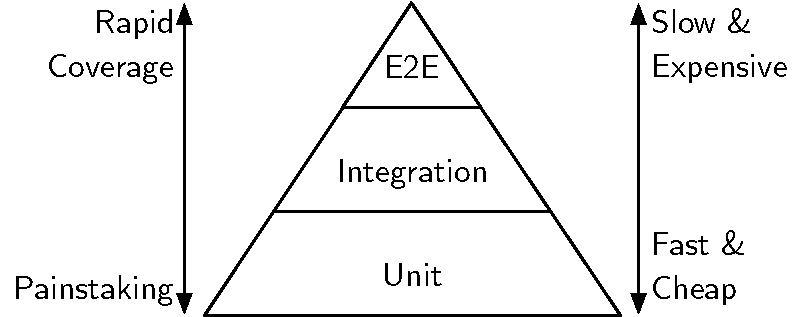
\includegraphics[width=25em]{test_pyramid}
  \caption{A view of the test pyramid.}%
  \label{fig:test_pyramid}
\end{wrapfigure}

In the case of software testing, the SUT can be different elements of a program, i.e.\ it can belong to different levels of abstraction.
One can decide to test a whole program, by manually giving inputs and verifying that the output is correct.
Or one could test individual functions, having a more control over the behaviour of each element.

These levels of test abstraction can be visualised with a test pyramid, as shown in \figurename~\ref{fig:test_pyramid}.
Tests are generally separated into three distinct categories.
The top category is for the End-to-End tests, which means testing the program as a whole.
It can mean interacting with the UI and evaluating the visual responses.
Whilst it allows for directly evaluating the well behaviour of the program, each test is costly in time and resources because the whole program has to be run.
Not only will each component be run, whether or not it requires testing, but time will also be spent on call to external libraries that are already tested.
At the other end of the test spectrum are the unit tests.
The goal is to test each and every component of the program (e.g.\ every function), as an individual and isolated from the rest of the program.
Running a single component is faster than running the whole program, but require much more work from the person writing tests, as every component needs its set of tests.
In between the two testing practices are the integration tests, which aim at ensuring the well collaboration of components \rephrase{work together as expected}, like verifying that gears rotate in the right way.
Examples of integration tests include API testing, or simply the fact of calling a function using the result from another function call.
This last example gives an intuition on how fuzzy the distinctions between all kinds of tests are, with definitions often relying on personal opinions\footnote{\url{https://testing.googleblog.com/2009/07/software-testing-categorization.html}}\footnote{\url{https://martinfowler.com/bliki/IntegrationTest.html}}.
More details about the loose definition of unit tests are given Section~\ref{sssec:unit_testing}.

The test hierarchy is often represented by a pyramid because it is generally advised to have many more unit tests than end-to-end tests.
Practitioners often recommend putting an emphasis on unit test, with a distribution of 70\% unit tests, 20\% integration tests, and 10\% end-to-end tests for example\footnote{\url{https://testing.googleblog.com/2015/04/just-say-no-to-more-end-to-end-tests.html}}.
More details on the strengths and weaknesses of unit tests are given in the next section, but we can convey some general truths here.
End-to-end tests require more maintenance as the software evolves, because test cases rely on many modules and their behaviour eventually change with time.
Also, with a broad coverage, it is difficult to identify components at fault in the case of a failing test.
Having unit tests for each component gives confidence that they behave accordingly and that if an integration test fails, the error lies in the interactions between the components.
Again, the broader the test, the greater the number of interactions which makes it difficult identifying the one at fault.
Because of this, the number of test levels has to increase alongside the software's growth --- e.g.\ grouping components into modules, modules into services, and services as the system.

Programs can be tested manually by a human (e.g.\ by interacting with the UI), but tests are generally automated to save time.
Automation often mean to programmatically describe a scenario, observations and their associated specifications.
Different levels can require different tools and frameworks\footnote{\url{https://martinfowler.com/articles/practical-test-pyramid.html}}.
For example, unit tests can be written in the same language as the main program, interacting with it like any other module (more details in the next section).
But to test a graphical user interface, one might need to run a window system and control the cursor's movements and clicks.

% - - - - - - - - - - - - - - - - - - - - - - - - - - - - - - - - - - - - - - - -
\subsubsection{Unit Testing}%
\label{sssec:unit_testing}

A unit test is supposed to target a precise component of the SUT, but defining the level of granularity is not trivial, even for experienced programmers\footnote{\url{https://martinfowler.com/bliki/TestPyramid.html}}\footnote{\url{https://martinfowler.com/bliki/UnitTest.html}}~\cite{runeson2006survey}.
In the case of a program written with an Object-Oriented language, such as Java --- we will put our focus on Java for the rest of this thesis --- the targeted component can be a class or just a method of a class.

\begin{listing}[H]
  \centering
  \begin{minted}[linenos,frame=topline,breaklines,highlightlines={3,5,7},highlightcolor=YellowOrange!20]{java}
public class TreeListTest {
    public void testIterationOrder() {
        TreeList tl = new TreeList(10);
        for (int i = 0; i < 10; i++) {
            tl.add(i);
        }
        ListIterator it = tl.listIterator();
  \end{minted}
  \begin{minted}[linenos,frame=bottomline,breaklines,firstnumber=last,highlightlines={11},highlightcolor=YellowGreen!20]{java}
        int i = 0;
        while (it.hasNext()) {
            Integer val = it.next();
            assertEquals(i++, val.intValue());
        }
    }
}
  \end{minted}
  \caption{Example of an object-oriented unit test (taken, and adapted for readability, from the Apache Commons Collections, in the class TreeListTest, line 270\protect\footnotemark): it consists of test inputs (lines 3--7) that manipulate the SUT\@; and assertions (line 11).\todo{what about lines 9 \& 10}}%
\label{lst:test_example}
\end{listing}
\footnotetext{\url{https://commons.apache.org/proper/commons-collections/xref-test/org/apache/commons/collections4/list/TreeListTest.html\#L271}}
\todo{the link might break in the future}
\todo{kinda assumes that \texttt{.hasNext()} and \texttt{.next()} are working properly}

An example of unit test is given in \listingname~\ref{lst:test_example}.
Tests are usually sorted in classes, and each test case corresponds to a method (which is why test cases are sometimes refered to as test methods, as we will encounter later on).
Specifications of expected values for observations are written using \emph{assertions}.
When the condition of an assertion is not met, we call it an assertion \emph{failure}, it raises an exception\rephrase{} and causes the test case to fail.
Assertions are a feature of test frameworks (i.e.\ internal DSL~\cite{fowler2010domain}), and allow test cases to be regular pieces of code.
This has advantages and disadvantages, it is easy to write test cases but might not be the most friendly\rephrase{} way to express a property on the software artifact targeted.
Test methods often rely on naming conventions to help the reader understand what is the target, and what behaviour it is checking.
Another pitfall to avoid is to test properties for the programming language used.

Unit tests are usually written by software engineers, as they are the one with the knowledge of the expected behaviour for the piece of software they have produced.
Large companies will also have test engineers, focusing on broader tests and commercially important features, as well as software engineers working on test infrastructure and tooling\footnote{\url{https://testing.googleblog.com/2016/03/from-qa-to-engineering-productivity.html}}.
Unit testing has becoming an integral part of modern software development with practices such as Test-driven Development (TDD)\footnote{\url{https://en.wikipedia.org/wiki/Test-driven_development}}~\cite{beck2003test} that consists in writing test cases first, and then writing code that complies.
Integrated development environments (IDEs) have been extended to make writing and reviewing tests easier.
Test automation in general is also a pillar of modern software delivery cycles like DevOps\footnote{\url{https://en.wikipedia.org/wiki/DevOps}}, with Continuous Integration (CI) tools that run test suites each time that code changes are pushed.
Tests can then be refined using exploratory testing\footnote{\url{https://testing.googleblog.com/2008/05/exploratory-testing-on-chat.html}}~\cite{kaner2000testing}, by trying to manually find flaws while documenting the process to then implement the results as test cases.
Manual testing is particularly useful to rapidly detect issues like slow response time, misleading error messages and other design concerns.

\begin{wrapfigure}[23]{R}{17em}
  \centering
  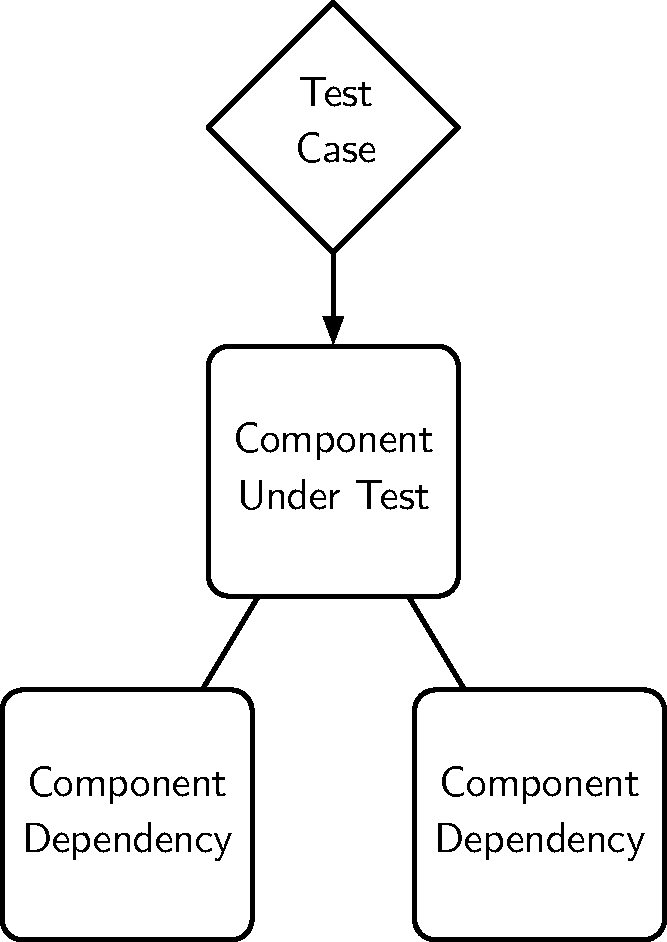
\includegraphics[width=17em]{component_dependency}
  \caption{Test target's dependencies.}%
  \label{fig:component_dependency}
\end{wrapfigure}

Because unit test are written with the same programming language as their target, certain features of the language --- that are supposed to help developers write clean code --- can become a hindrance.
A perfect example with Java are the private methods.
They exist because they enforce the separation of the public interface and the inner workings of a class.
But when one want to test a private method to make sure it does the right thing, it is not possible.
The alternative is to extensively test the public methods, making sure they trigger all sorts of behaviour in the private part of the class.
In this situation, we end testing a component that interacts with other components, as depicted in \figurename~\ref{fig:component_dependency}, but then it becomes a small integration test\footnote{\url{https://martinfowler.com/bliki/UnitTest.html}}.
The granularity of tests does not only depend on the needs and desires of the developer, but also on the limitations of the language.
Object-Oriented are particularly victim to this, as they are suited for composition design patterns~\cite{wolfgang1994design}, leaving no other option to the developer to try to limit interactions.
Ways to avoid writing test that trigger a long chain of reactions is to use doubles (or mocks) which are hand written clones of classes instances.\rephrase{}

Another common problem with testing are flaky tests.
A flaky test is a test which result is not deterministic.
There can be various causes for a flaky test, e.g.\ a direct usage of RNG function, or a crash happening only in scenario with a certain scheduling in the case of parallel applications.
The advantage of small tests with controlled interaction with the environment is that they are less likely to be flaky.
This a hard problem\footnote{\url{https://testing.googleblog.com/2017/04/where-do-our-flaky-tests-come-from.html}} as flaky tests can be (i) hard to identify, (ii) hard to refactor, and (iii) hard to avoid in the first place.

\todo{unit tests also make up for examples in OSS}

\todo{how do you know you have a good oracle}

% --------------------------------------------------------------------------------
\subsection{Elementary Metrics}%
\label{ssec:elementary_metrics}
Metrics have been developed to help developers automatically assess the quality of their code.
Each metric measures one specific characteristic, such as the need for refactoring, the size of the program, or --- and we are particularly interested in this one --- the likelihood of bugs.

\begin{figure}
  \centering
  \fbox{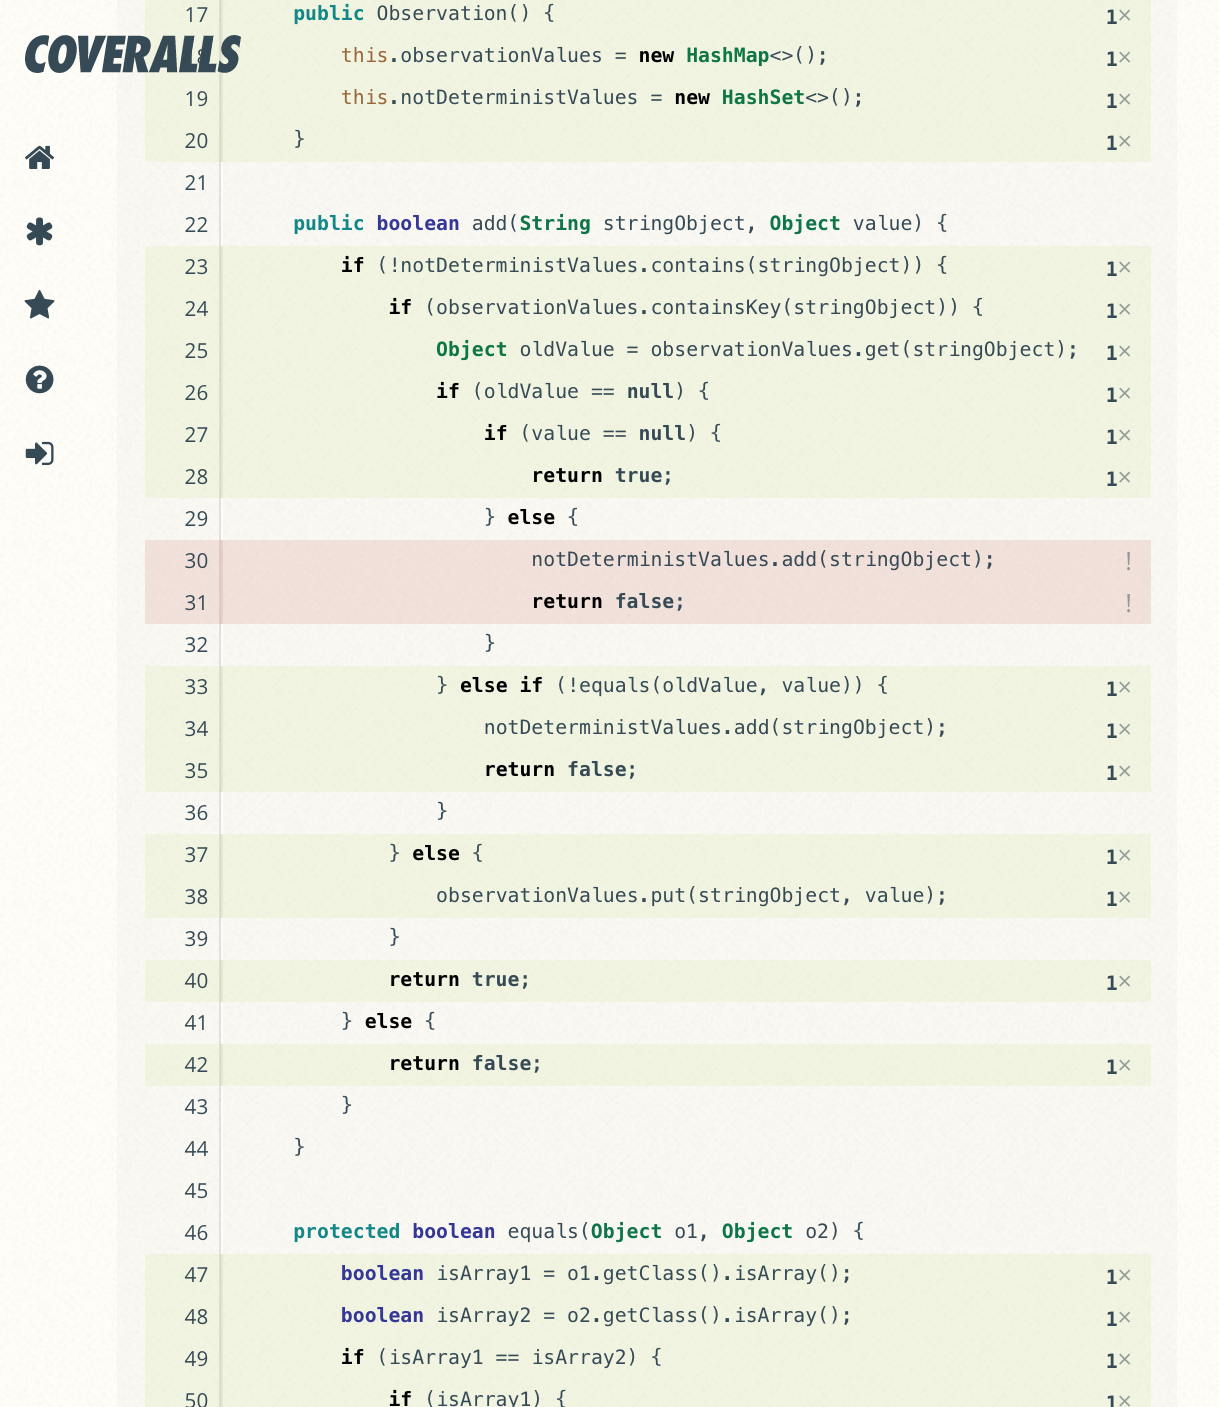
\includegraphics[scale=0.80, trim=5.1cm 4.3cm 1.5cm 3.7cm, clip]{screenshot_coverage}}
  \cprotect\caption{Example of coverage reporting from the Coveralls\protect\footnotemark{} tool. We can see that the statements in the first \texttt{else} branch have not been executed a single time}%
  \label{fig:screenshot_coverage}
\end{figure}
\footnotetext{\url{https://coveralls.io/}}

The most basic metrics to measure how thoroughly tested a system is, are coverage based metrics.
For example, during the test suite execution, one can keep track of all statements that were executed.
At the end, you have a percentage of executed statements for the total number of statements.
Instead of statements, one can also keep track of control flow branches explored.
\todo{give examples for other metrics?}
These metrics, especially the statement coverage, are wide spread in the industry --- with coverage tools integrated out-of-the-box with source code hosting services and continuous integration services.
An example of coverage visual report is shown in \figurename~\ref{fig:screenshot_coverage}.

It is generally acknowledged that a system with high coverage means that the system is less likely to have bugs --- but it is not foolproof~\cite{hovemeyer2004finding,inozemtseva2014coverage}.
Such simple metrics are not good at pointing out corner cases.
If we take the following example \texttt{if ($C_1$ AND ($C_2$ OR $C_3$))} and $C_3$ makes the program crash, then it is possible the explore both branches without executing $C_3$.
\todo{What are their limits}

A drawback of metrics is that in practice, testers will change behaviour once they know how the measurement works\footnote{\url{https://testing.googleblog.com/2009/09/7th-plague-and-beyond.html}}.
They will write tests that will perform well for a given metric and ignoring other important factors (e.g.\ diversity\footnote{\url{https://testing.googleblog.com/2009/06/by-james.html}}~\cite{baudry2014diversify,baudry2015multiple}).
In these cases the metric has become the goal instead of a progress measurement.

% --------------------------------------------------------------------------------
\subsection{Mutation Testing}%
\label{ssec:mutation_testing}
\begin{wrapfigure}[23]{L}{9em}
  \centering
  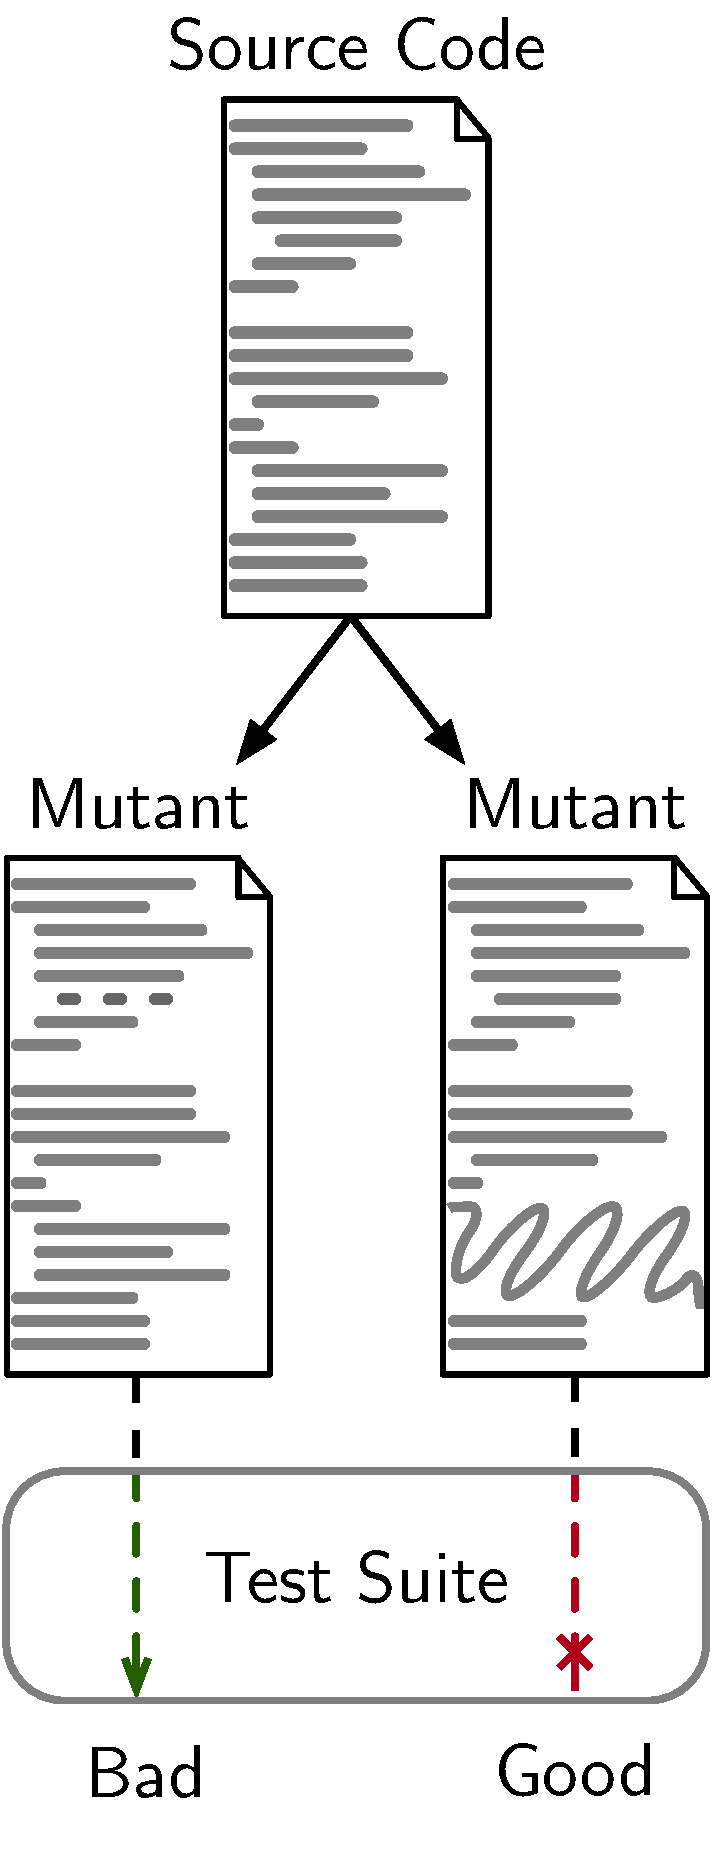
\includegraphics[width=9em]{mutation_testing_report}
  \caption{Mutation testing process.}%
\label{fig:mutation_testing}
\end{wrapfigure}
% Introduction
Mutation testing is a method used to assess the quality of a test suite, giving it a grade called \textit{mutation score}.
The idea is to insert bugs in the software and see if these faulty versions still pass the tests or not.
We call the derived versions \textit{mutants}, hence the name mutation testing.
When a mutant goes through the test suite without making a single test fail, it is considered \emph{live}, and the opposite case it is considered \emph{dead}.
The global process is depicted in~\figurename~\ref{fig:spaces}.
The main appeal is that, a test suite with a good mutation score, in addition to ensure the well behaviour of the SUT in useful scenarios, it can detect bad behaviours --- which is particularly useful for regression testing.
\todo{rework that sentence}
There is a correlation between mutation score and coverage score as test suites with high mutation score tend to have good coverage~\cite{assylbekov2013investigating}.
It has been found that correlations between mutation scores and real fault detection are weak~\cite{papadakis2018mutation,just2014mutants}.

\todo{a mutation covered line is stronger than a regular covered line}

\addref{fundational papers}

\todo{mutation testing has been extended in various directions, e.g.\ specification mutation, but we are focusing on the primary usage, the evaluation of test suites and the implementation}

% Mutators
Mutants are obtained by applying \emph{mutators} on the original version.
These operators can be varied, from fine grained like changing a condition (e.g.\ substituting $\leq$ with $>$), to the granularity of classes~\cite{segura2011mutation} (e.g.\ delete the body of a method \addref{descartes}).
Running first mutation testing with large operators allows to rapidly detect gaps in the coverage of the test suite for unit testing but also for integration testing.
Fine grained mutation can then be employed to meticulously evaluate the functional testing capabilities of the test suite~\cite{howden1982weak}.
Most of the time, we generate 1-\emph{order} mutants, that means that a mutant is the result of a mutator applied once.
A mutator will usually generate several mutants.
For example, a mutator that replaces a \texttt{while} statement into a \texttt{do-while} statement will generate a mutant for each \texttt{while} in the artifact.
In the case of $k$-order mutants, which can be thought of as the result of $k$ succesive 1-order mutants\cite{wah2000theoretical}, the number of derived programs starts to blow up.

% Difficulties
Mutation testing suffers from drawbacks that have limited its use outside of the research world even though it has been an active research domain for many years~\cite{jia2011analysis}.
The first obvious flaw is that it is slow.
For compiled languages, all mutants have to be compiled, and that process often takes a lot of time for large programs.
Then the whole test suite has to be executed for each mutant, which again is a long process.
However, given certain trade-offs in terms of quality of the mutation analysis process (e.g.\ not generating all possible mutants), the computational complexity can be dodged~\cite{offutt1993experimental,movzucha2016mutation}.
Optimized techniques for regression testing also exist~\cite{yoo2012regression}, including minimisation, selection and prioritisation, which can reduce the execution time of the test suite.
The mutant generation is also full of traps.
The major pitfall that cannot be avoided is the equivalent mutant problem.
Some mutants, although they have a different program than the original, have the same semantics.
Which means that they will always pass the test suite and will not bring any insight on the SUT\@.
The generation of mutants that are simply syntactically valid is also a non-trivial problem that requires pattern replacement instead of simple text replacement~\cite{simao2009transformational}.

Another difficulty for mutation testing to take on in the industry is the lack of understanding by practitioners.\todo{rework that sentence}
The process of mutation and elimination can be confusing.
But also, when a mutant is live, it is not always clear what actions should be taken in order to kill it.
\todo{maybe add more}
\todo{teaching mutation testing using gamification}

% Pitest
Multiple mutation tools exist, with differences on the level of abstraction they handle, different performances and different correlation with real fault detection.
Many of them are robust thanks to the efforts from the research community to reach the industry and the need to have reliable implementations to do\rephrase{} empirical studies related to mutation testing.
One of these tools is PIT\footnote{\url{http://pitest.org/}}~\cite{coles2016pit}, a tool for the Java bytecode.
The research version (i.e.\ state-of-the-art) of PIT is known to perform better than its competitors overall~\cite{kintis2017effective}.
Two technical details are interesting for us.
The first one is the way it stores the mutants generated.
\todo{}
The other important detail is that PIT is deterministic.
That is, for the same program, the same mutants will always be generated, and thus the mutation score will always be the same.

\begin{figure}
  \centering
  \fbox{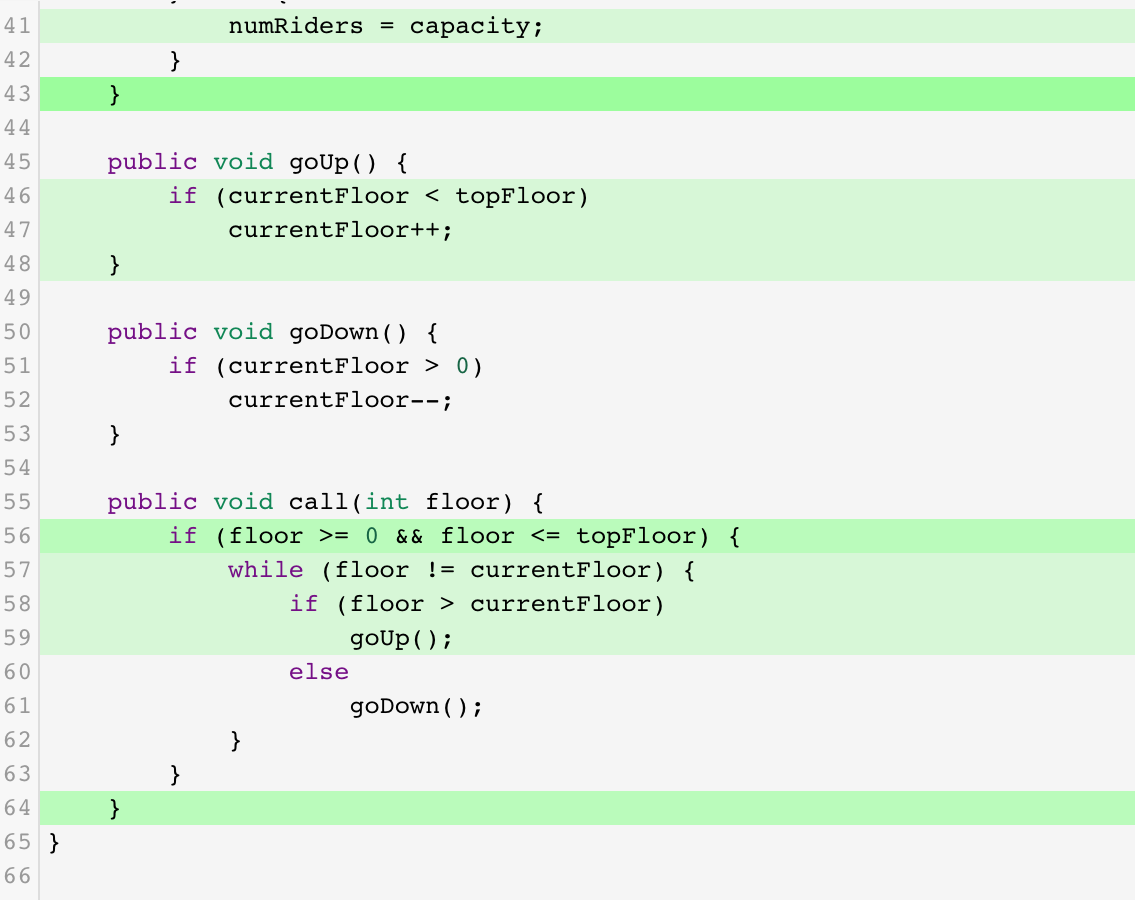
\includegraphics[scale=0.75,trim=0cm 1.4cm 6.7cm 8.6cm, clip]{screenshot_mutation_coverage}}
  \caption{Example of mutation coverage reporting from Code Defenders\protect\footnotemark{}~\cite{rojas2017code}. Shades of green are used to denote the amount of testing for a line.}%
  \label{fig:screenshot_mutation_coverage}
\end{figure}
\footnotetext{\url{http://code-defenders.org/}}
The way mutation testing tool report their result is interesting.
Instead of trying to shown each statement that has been mutated, and inspired by reports of line coverage, they usually display a regular line coverage report with shades of colour.
The lightest means that the line has been executed, and the darker it gets, the higher the number of mutants located in this line.
An example of mutation coverage visual report is shown in \figurename~\ref{fig:screenshot_mutation_coverage}.

% --------------------------------------------------------------------------------
\subsection{The Need for Easy-to-use Tools}%
\label{ssec:need_easy}
\todo{easy to understand}
\todo{useful for surveys}
\cite{delahaye2015selecting}

\todo{tests are written by regular developers, even though there are engineers specialised in testing\footnote{\url{https://testing.googleblog.com/2016/03/from-qa-to-engineering-productivity.html}}}
\todo{hard to move the industry forward}
\todo{we share similar experience with static analysis tool researchers}
\todo{avoid false positives, angry developers, must feel they benefit from the tool, enjoy using it~\cite{bessey2010few,sadowski2018lessons}}
\todo{\emph{effective false positives}~\cite{sadowski2015tricorder}}

% --------------------------------------------------------------------------------
\subsection{Cognitive Support Tool Development}%
\label{ssec:cognitive_support}
\todo{}
\cite{oviatt2006human}
\cite{stol2016grounded}

\todo{case studies~\cite{flyvbjerg2006five}}


% ================================================================================
\section{Test Suite Amplification}%
\label{sec:test_suite_amplification}
In this Section, we provide more context for this thesis' contribution.
We explain how global optimization techniques, including metaheuristic search techniques (e.g.\ genetic algorithms) can be applied to software engineering problems --- for example, by using software metrics as target functions.
Section~\ref{ssec:genetic_improvement} presents how source code can be manipulated for search processes, and Section~\ref{ssec:test_amplification} presents the specific problem of improving test suites.
Section~\ref{ssec:dspot} introduces~\dspot{}, a tool that enhances tests for a better coverage, and for which this thesis can be seen as an extension.\rephrase{}

% --------------------------------------------------------------------------------
\subsection{Genetic Improvement}%
\label{ssec:genetic_improvement}
\todo{}

Genetic improvement (GI)~\cite{petke2017genetic} uses automated search \todo{explain what automated search is} to find improved versions of existing software.
Applying search-based techniques for software engineering problems is not new~\cite{mcminn2011search} as is the field of genetic programming (GP)~\cite{koza1994genetic}.
But since\rephrase{} the name of GI has been coined in 2012~\cite{harman2012gismoe}, the level of computing power reached has allowed research to achieve impressive results.

\addref{fundational papers}

\addref{the surprising creativity of digital evolution?}

Search operators are most frequently \emph{delete}, \emph{copy} and \emph{replace}~\cite{petke2017new}.
\todo{}

% --------------------------------------------------------------------------------
\subsection{Test Amplification}%
\label{ssec:test_amplification}
As unit tests are program artefacts like others, GI can be applied on test suites~\cite{danglot2017emerging}\addref{A Systematic Literature Review on Test Amplification} and search techniques have been employed since 2005~\cite{baudry2005automatic}.
It is relatively recent compared to works tackling the problem of Test Data Generation (i.e.\ generating tests from scratch for a piece of software), but it is only recent that we can expect software projects, large or modest, to come with strong test suites.
Various goals can be pursued to improve a test suite, from automated refactoring to improve a specific metric, to enhancement of existing tests to fill the often partial coverage\footnote{\url{https://testing.googleblog.com/2014/07/measuring-coverage-at-google.html}}.
The term of test \emph{amplification} is used to denote the process of processing and extending tests to reach further targets.
Baudry et al.~\cite{baudry2005automatic} wrote a tool for C\#\rephrase{} to explore more of the input space and improve the mutation score.
Yoo et al.~\cite{yoo2012test} proposed the Test Data Regeneration (TDR) method for creating equivalent tests with different inputs --- particularly useful for fault detection and avoiding overfitting\todo{explain overfitting}.
Xuan et al.~\cite{xuan2015dynamic,xuan2016b} created a tool to refactor test suite to improve dynamic analysis and fault detection.

% --------------------------------------------------------------------------------
\subsection{\dspot{}}%
\label{ssec:dspot}

\begin{figure}
  \centering
  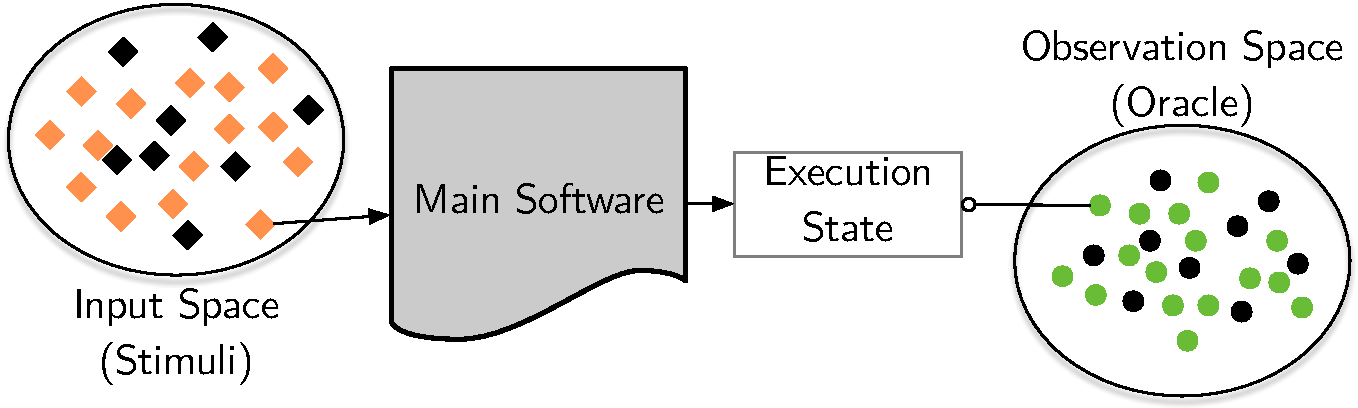
\includegraphics[width=36em]{spaces_report}
  \caption{On the left, the testing input space is composed by specified input points (orange diamonds) and unspecified input points (black diamonds). On the right, the observation space over a given program state depicts the assertions of tests. The green circles are values that are already asserted in the existing test suite, the newly added assertions are shown as black circles.}%
\label{fig:spaces}
\end{figure}

\dspot{}\footnote{\url{https://github.com/STAMP-project/dspot}}\addref{Genetic-Improvement based Unit Test Amplification for Java}\cite{baudry2015automatic,baudry2014tailored,baudry2015dspot} is a test amplification tool.
Its goal is to amplify tests individually to improve a given metric, e.g.\ mutation score.
Going back to our definition of tests, with the notions of stimuli and observations, \dspot{} has a search process on both spaces.
New inputs are generated, and new observations are made.
A visual representation is given in \figurename~\ref{fig:spaces}.
Because of the oracle problem, \dspot{} focuses on regression testing --- assertions (i.e.\ specifications) are generated from observations of an actual execution of the test.
It is a Java tool and it uses Spoon~\cite{pawlak2016spoon} to manipulate the source code.

To explore more of the input space (we also talk about \emph{amplifying} inputs), operators called I-Amplification are applied.
\begin{description}
  \item[\textit{Amplification of literals}] Similarly to TDR, literals (numeric, boolean, string) are replaced by neighbours. For example, an integer can be multiplied by 2 or a random character can be added to a string.
  \item[\textit{Amplification of method calls}] Methods calls can be duplicated, removed, or made-up by picking a random variable in the test and calling one of its methods with random parameters.
  \item[\textit{Test objects}] If a new object is required for an amplified method call, one of the appropriate type will be built by using the default constructor.
\end{description}
Like 1-order mutants, only one amplification is applied at a time, to limit the number of generated tests.
Because the random amplification can create flaky tests, they are executed three times to verify that they have a consistent behaviour.

As for the amplification of observations (A-Amplification), focus is put on checking more properties to kill more mutants.
Assertions are generated as follows: the state of program is collected after execution of the test case to know the actual values and use these values as oracle.

\dspot{} is different from traditional test generator like EvoSuite~\cite{fraser2011evosuite} for multiple reasons.
It is more than just using the existing test suite as a good starting population.
\todo{}

The result of \dspot{} is a set of amplified tests but it should not stop there.
Building incrementally on top of humans work is valuable.
Adding the generated tests in the main test suite has multiple advantages.
First, is the review process.
Developers have to review changes before it is accepted in the main code.
During the review process developers can tweak the assertions, rearrange the inputs, etc.
In that sense, \dspot{} fits as a software development bot, integrated in the workflow~\cite{urli2018design}, that could be run on code changes, after making sure the tests suite is passing.
Secondly, it is more efficient.\todo{}


% ================================================================================
\section{Problem Statement}%
\label{sec:problem_statement}
This thesis aim at helping developers understand amplified tests.
There are two sides for this problem: supporting the developer understand the test (Section~\ref{ssec:need_doc}) and cleaning the tests from the noise injected during the amplification process (Section~\ref{ssec:random_noise}).

\todo{understanding the test is essential~\cite{bessey2010few,sadowski2018lessons}}
\todo{important for maintenance when a test comes to fails, to build trust in the tool, etc.}

\addref{How Do Automatically Generated Unit Tests Influence Software Maintenance?}

% --------------------------------------------------------------------------------
\subsection{The Need for Unit Test Cases Documentation}%
\label{ssec:need_doc}
\todo{}
Several works have highlighted the need for test documentation~\cite{prado2015wap,prado2016advances,prado2018towards,li2016automatically,daka2014survey,panichella2016impact}.

\todo{tests are complex}

\todo{lack of why information}

\todo{the code the test interacts with; what the code does; what is expected}

\todo{programmers like short textual description}

\todo{explain what li2016automatically has done}

\todo{talk about the field of software maintenance~\cite{swanson1976dimensions}}

\todo{lack of work on generating human friendly descriptions for mutation testing}

% --------------------------------------------------------------------------------
\subsection{The Generated Random Noise}%
\label{ssec:random_noise}
\todo{}

\todo{One problem shared with test generation from scratch is that it's hard to understand the test, it's messy}


% ================================================================================
\section{Related Works}%
\label{sec:related_works}
\todo{}

% --------------------------------------------------------------------------------
\subsection{Automatic Test Case Documentation}%
\label{ssec:test_doc}
\todo{}

\todo{paraphrasing the code; lack of why information}

\todo{stereotypes are for general purpose code}

\cite{neubig2016survey,nazar2016summarizing,li2016automatically,li2018automatically,kamimura2013towards,ghafari2015automatically}

\todo{there are also works on documenting code changes (i.e.\ commits)}
\cite{cortes2014automatically,linares2015changescribe,dragan2011using,jiang2017towards,jiang2017automatically,shen2016automatic,buse2010automatically}
\todo{machine learning neural network~\cite{loyola2017neural}}
\todo{purely what information, characterizing the mechanisms of change~\cite{buckley2005towards}}

\todo{works on describing code written by humans~\cite{wang2018comment,dragan2006reverse,dragan2011emergent,moreno2012jstereocode,buse2008automatic,sridhara2010towards,herbert2016swummary,mcburney2016automatic,sridhara2011automatically,moreno2013automatic} (e.g.\ mining comments, method and class stereotypes (too general purpose), summary, simple (syntactic) context, nl paraphrasing)}

\todo{Automatic summarization of natural language documents has been attempted by researchers for more than half a century~\cite{jones2007automatic}}


\todo{fully fledged GUI on method execution report~\cite{beck2017method} fully fledged GUI for mutants~\cite{delamaro2001proteum} providing information on mutant and test case}

% --------------------------------------------------------------------------------
\subsection{Cognitive Support for Unit Testing Review}%
\label{ssec:cognitive_support_unit_test}
\todo{}

% --------------------------------------------------------------------------------
% \subsection{Source Code Change Documentation}%
% \label{ssec:commit_generation}
% \todo{}


% ================================================================================
\section{Contribution}%
\label{sec:contribution}
\todo{}

% --------------------------------------------------------------------------------
\subsection{Identifying Amplifications}%
\label{ssec:retrieve_amplifications}
\todo{}

% --------------------------------------------------------------------------------
\subsection{Minimisation}%
\label{ssec:minimisation}
\todo{}
\todo{put slicing before?}

\todo{removing useless assertions}

\todo{cannot use general purpose techniques\cite{leitner2007efficient,zeller1999yesterday} because we want the original part intact?}

% --------------------------------------------------------------------------------
\subsection{Replace or Keep}%
\label{ssec:replace_keep}
\todo{}

% --------------------------------------------------------------------------------
\subsection{Focus}%
\label{ssec:focus}
\todo{}
\cite{liu2006approach}

% --------------------------------------------------------------------------------
\subsection{Slicing}%
\label{ssec:slicing}
\todo{}
\cite{dolby2015tj}\footnote{\url{http://wala.sourceforge.net/}}

% --------------------------------------------------------------------------------
\subsection{Natural Language Description}%
\label{ssec:nl_description}
\todo{}

\todo{Focus on mutation testing}

\todo{avoid talking about mutants}
\todo{How to describe a mutant}

\todo{SWUM~\cite{hill2010integrating}}
\cite{alali2008s,hattori2008nature,letovsky1987cognitive}

\todo{what informations we have at our disposal: original test, amplified test, tagged amplified nodes}

List of possible information:
\begin{itemize}
  \item control flow branches
  \item name of mutant
  \item code under test~\cite{qusef2011scotch}
  \item traceability link
  \item label/stereotype
\end{itemize}

\todo{on the usefulness of nlg}

% --------------------------------------------------------------------------------
\subsection{Ranking}%
\label{ssec:ranking}
\todo{}


% ================================================================================
\section{Evaluation}%
\label{sec:eval}
\todo{}

% --------------------------------------------------------------------------------
\subsection{Threat to Validity}%
\label{ssec:threat_to_validity}
\todo{}

\todo{DSpot is not yet established and recognized in the community. It is is difficult to have input data (valid amplified tests)}

% --------------------------------------------------------------------------------
\subsection{Case Studies}%
\label{ssec:case_studies}
\todo{}

% --------------------------------------------------------------------------------
\subsection{Performances}%
\label{ssec:performances}
\todo{}


% ================================================================================
\section*{Conclusion}%
\label{sec:conclu}%
\addcontentsline{toc}{section}{\nameref{sec:conclu}}
\todo{}


% ================================================================================
\section*{Acknowledgments}%
\label{sec:ack}%
\addcontentsline{toc}{section}{\nameref{sec:ack}}
Thanks to Benoit Baudry and Martin Monperrus for their guidance.
Thanks to Benjamin Danglot for his collaboration and all his work on \dspot.
Thanks to Zimin Chen, Nicolas Harrand, He Ye and Long Zhang for making daily life enjoyable.
This internship was supported by the Fondation Rennes 1 and its patrons.
Many thanks to KTH for hosting me.


% ================================================================================
\bibliographystyle{ieeetr}%
\bibliography{../bibl}
\addcontentsline{toc}{section}{References}

\end{document}
